\cleardoublepage

%\ifpdf
%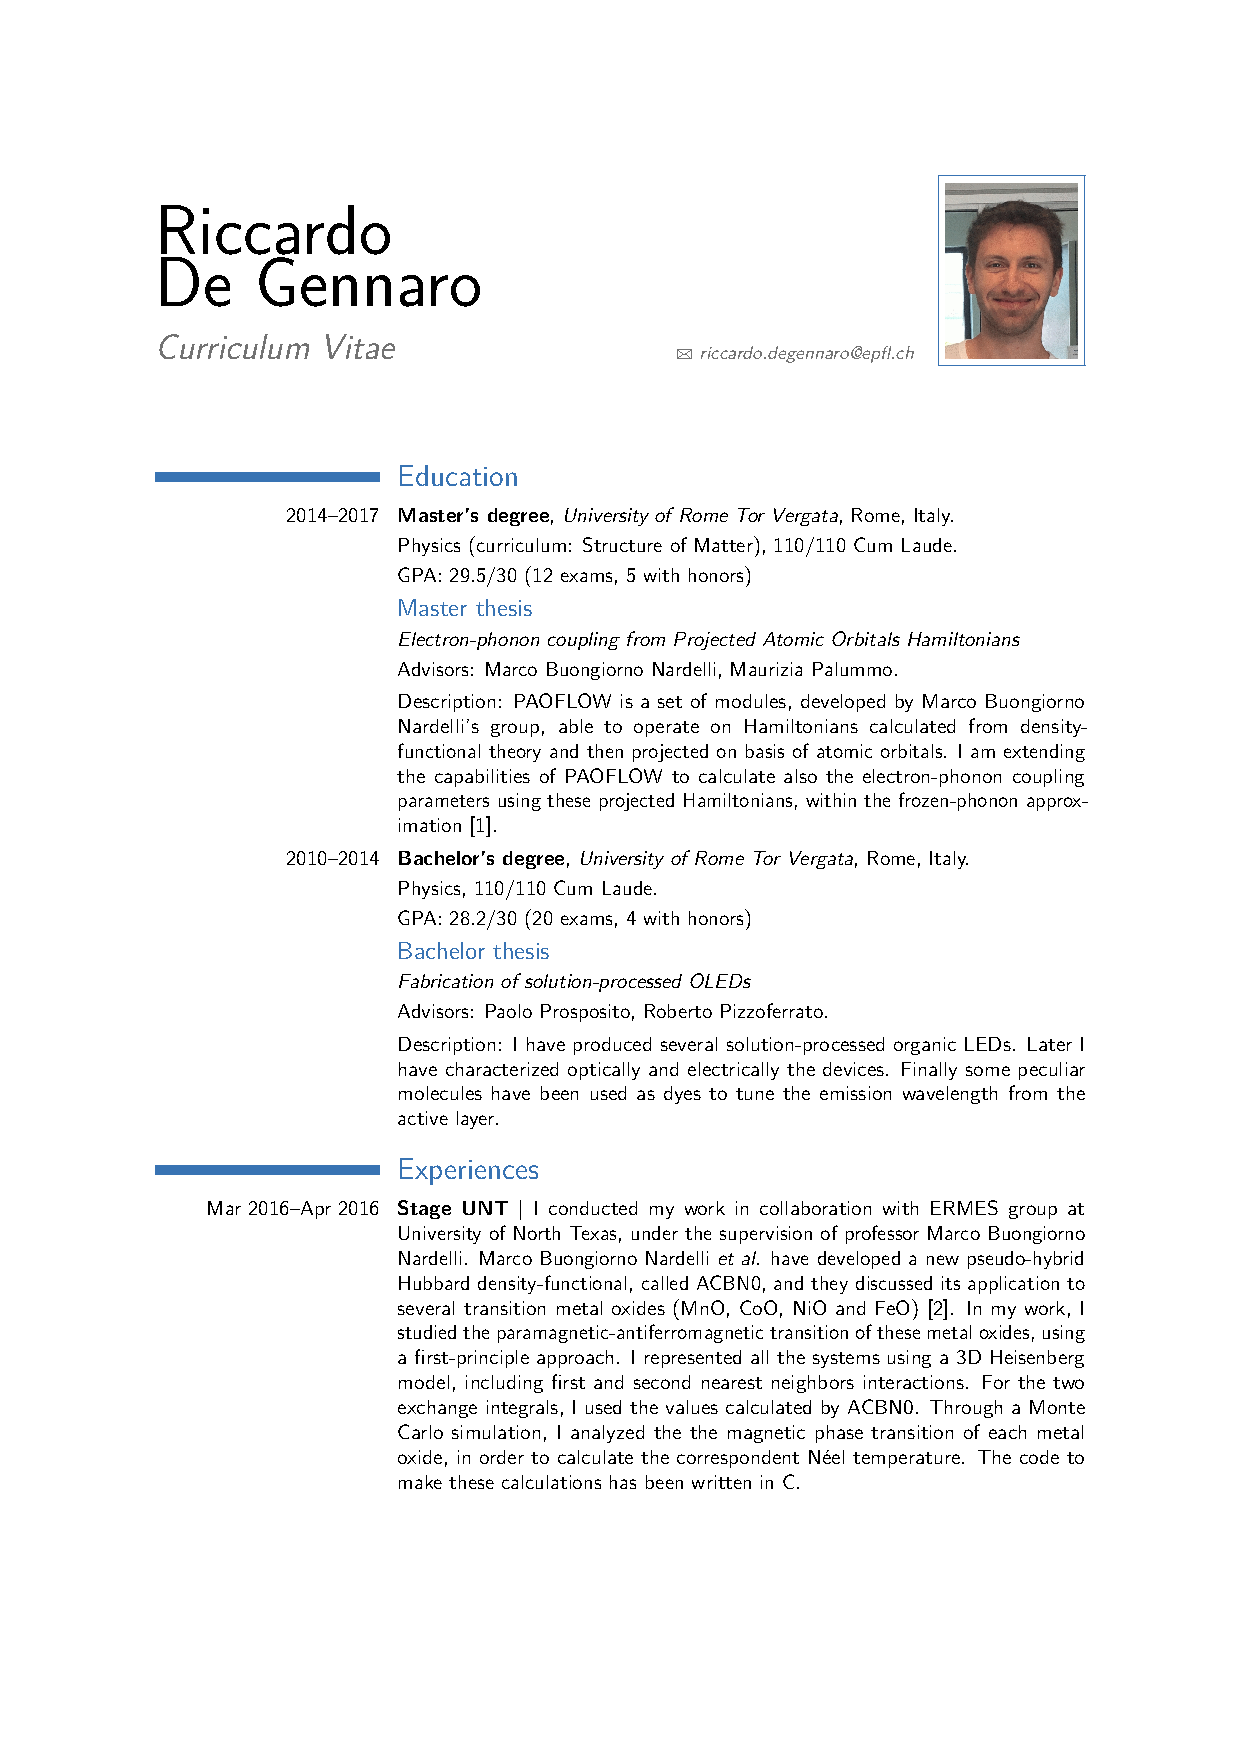
\includepdf[pagecommand=\thispagestyle{addpagenumbersforpdfimports},pages=-]{tail/cv.pdf}
%\fi


\chapter{Curriculum Vitae}
\phantomsection
%\addcontentsline{toc}{chapter}{Curriculum Vitae}
\markboth{Curriculum Vitae}{Curriculum Vitae}

\section*{Personal data}

\begin{tabular}{p{5cm}l}
    Name                    & Riccardo De Gennaro \\
    Date and place of birth & 05.09.1991 in Rome (Italy) \\
    Citizenship             & Italian \\
    Email                   & \href{mailto:riccardo.degennar@gmail.com}{riccardo.degennar@gmail.com}
\end{tabular}

\section*{Education}

\begin{tabular}{p{.15\linewidth}p{.85\linewidth}}
    2018 -- 2022 & PhD in Materials Science, \epfl (EPFL) \\
                 & PhD thesis: \emph{Spectral properties of extended systems from Koopmans-compliant functionals} (supervisors: Prof. \director, Dr. \codirector)\\
    2014 -- 2017 & MSc in Physics (Structure of Matter), \uniroma \\
                 & MSc thesis: \emph{Electron-phonon coupling from projected atomic orbitals Hamiltonians} (supervisors: Prof. Marco Buongiorno Nardelli, Prof. Maurizia Palummo) \\
    2016 -- 2017 & 5-month exchange student, \unt (UNT) \\
                 & MSc thesis and MSc project \\
    2010 -- 2014 & BSc in Physics, \uniroma \\
                 & BSc thesis: \emph{Fabrication of solution-processed OLEDs} (supervisors: Prof. Paolo Prosposito, Prof. Roberto Pizzoferrato)
\end{tabular}

\section*{Publications related to the thesis}

\begin{itemize}
    \item E. Linscott, N. Colonna, R. De Gennaro, and N. Marzari, \emph{koopmans: an open-source package for performing Koopmans spectral functional calculations} (to be submitted)
    \item N. Colonna, R. De Gennaro, E. Linscott, and N. Marzari, \emph{Koopmans Spectral Functionals in Periodic Boundary Conditions}, \href{https://doi.org/10.1021/acs.jctc.2c00161}{J. Chem. Theory. Comput. \textbf{18}, 5435 (2022)} \vfill
    \item R. De Gennaro, N. Colonna, E. Linscott, and N. Marzari, \emph{Bloch's theorem in orbital-density-dependent functionals: Band structures from Koopmans spectral functionals}, \href{https://link.aps.org/doi/10.1103/PhysRevB.106.035106}{Phys. Rev. B \textbf{106}, 035106 (2022)}
    \item M. Puppin, S. Polishchuk, N. Colonna, A. Crepaldi, D. N. Dirin, O. Nazarenko, R. De Gennaro, G. Gatti, S. Roth, T. Barillot, L. Poletto, R. P. Xian, L. Rettig, M. Wolf, R. Ernstorfer, M. V. Kovalenko, N. Marzari, M. Grioni, and M. Chergui, \emph{Evidence of Large Polarons in Photoemission Band Mapping of the Perovskite Semiconductor $CsPbBr_3$}, \href{https://link.aps.org/doi/10.1103/PhysRevLett.124.206402}{Phys. Rev. Lett. \textbf{124}, 206402 (2020)}
\end{itemize}

\section*{Other publications}

\begin{itemize}
    \item C. Toher \emph{et al.}, \emph{The AFLOW Fleet for Materials Discovery}, \href{https://doi.org/10.1007/978-3-319-44677-6_63}{In: W. Andreoni, S. Yip, (eds) Handbook of Materials Modeling, Springer, Cham (2020)}
    \item M. Buongiorno Nardelli, F. T. Cerasoli, M. Costa, S. Curtarolo, R. De Gennaro, M. Fornari, L. Liyanage, A. R. Supka, H. Wang, \emph{PAOFLOW: A utility to construct and operate on ab initio Hamiltonians from the projections of electronic wavefunctions on atomic orbital bases, including characterization of topological materials}, \href{http://www.sciencedirect.com/science/article/pii/S0927025617306651}{Comput. Mater. Sci. \textbf{143}, 462 (2018)}
    \item P. Gopal, R. De Gennaro, M. Gusmao, R. A. R. A. Orabi, H. Wang, S. Curtarolo, M. Fornari, and M. Buongiorno Nardelli, \emph{Improved electronic structure and magnetic exchange interactions in transition metal oxides}, \href{https://doi.org/10.1088%2F1361-648x%2Faa8643}{J. Phys.: Condens. Matter \textbf{29}, 444003 (2017)}
\end{itemize}

\section*{Contributed talks at international conferences}

\begin{itemize}
    \item R. De Gennaro, N. Colonna, E. Linscott, N. Marzari, \emph{Defect levels in doped silicon using Koopmans spectral functionals}, \href{https://meetings.aps.org/Meeting/MAR22/Session/A48.11}{APS March Meeting 2022, A48.00011}
    \item R. De Gennaro, N. Colonna, N. Marzari, \emph{Band structure of semiconductors and insulators from Koopmans-compliant functionals}, \href{https://meetings.aps.org/Meeting/MAR21/Session/M22.4}{APS March Meeting 2021, M22.00004}
\end{itemize}

\section*{Participation at other events}

\begin{itemize}
    \item \href{https://www.psik2022.net/home}{\emph{Psi-k Conference}}, Poster Commendation, 22-25 August 2022, Lausanne
    \item \href{https://sites.google.com/view/etsfyrm2021}{\emph{17th ETSF Young Researchers' Meeting}}, Organizer of the conference, 6-10 September 2021, Cagliari
    \item \href{https://indico.ictp.it/event/9018/}{\emph{Computational School on Electronic Excitations in Novel Materials Using the Yambo Code}}, 27-31 January 2020, Trieste
    \item \href{https://psi-k.net/report-on-quo-vadis-self-interaction-correction-qvsic-september-23-26-2019-freiberg-germany/}{\emph{Quo vadis self-interaction correction?}}, 23-26 September 2019, Freiberg
    \item \href{https://sites.google.com/view/eth-electronic-structure-2019}{\emph{Advanced Electronic Structure Methods in Condensed Matter Physics}}, 8-10 July 2019, Lausanne
    \item \href{https://www.etsf.eu/node/113}{\emph{16th ETSF Young Researchers' Meeting}}, 3-7 June 2019, San Sebasti\'{a}n
    \item \href{https://indico.ictp.it/event/8658/}{\emph{19th International Workshop on Computational Physics and Material Science: Total Energy and Force Methods}}, 9-11 January 2019, Trieste
    \item \href{https://sites.google.com/view/comdi2018/home?authuser=0}{\emph{International Workshop on Computational Design and Discovery of Novel Materials}}, 10-12 September 2018, Lausanne
    \item \href{https://www.sps.ch/en/events/sps-annual-meeting-2018/}{\emph{SPS Annual Meeting}}, 28-31 August 2018, Lausanne
    \item \href{https://www.cecam.org/workshop-details/238}{\emph{Bandstructure meets quantum field theory}}, 2-6 July 2018, Vienna
\end{itemize}
